\documentclass[12pt,a4paper]{report}

% ============================
% Packages
% ============================
\usepackage[a4paper,margin=2.5cm]{geometry}
\usepackage[T1]{fontenc}
\usepackage[utf8]{inputenc}
\usepackage{lmodern}
\usepackage{microtype}
\usepackage{setspace}
\usepackage{graphicx}
\usepackage{booktabs}
\usepackage{tabularx}
\usepackage{longtable}
\usepackage{array}
\usepackage{amsmath}
\usepackage{amssymb}
\usepackage{xcolor}
\usepackage{hyperref}
\usepackage{fancyhdr}
\usepackage{caption}
\usepackage{subcaption}
\usepackage{tikz}
\usetikzlibrary{positioning,arrows.meta}
\usepackage{listings}
\usepackage{tcolorbox}
\tcbuselibrary{skins,breakable,listings,theorems}
\usepackage{float}

% ============================
% Styling
% ============================
\onehalfspacing

\definecolor{brandBlue}{HTML}{1D4ED8}
\definecolor{brandTeal}{HTML}{0F766E}
\definecolor{brandAmber}{HTML}{B45309}
\definecolor{brandRed}{HTML}{B91C1C}
\definecolor{brandGray}{HTML}{111827}
\definecolor{softBlue}{HTML}{EFF6FF}
\definecolor{softTeal}{HTML}{ECFDF5}
\definecolor{softAmber}{HTML}{FFFBEB}
\definecolor{softRed}{HTML}{FEF2F2}

\hypersetup{
  colorlinks=true,
  linkcolor=brandBlue,
  urlcolor=brandTeal,
  citecolor=brandAmber
}

\pagestyle{fancy}
\fancyhf{}
\lhead{Metin2 Market Data Warehouse}
\rhead{\thepage}
\renewcommand{\headrulewidth}{0.4pt}

% ============================
% Listings
% ============================
\lstdefinestyle{python}{
  language=Python,
  basicstyle=\ttfamily\small,
  keywordstyle=\color{brandBlue}\bfseries,
  commentstyle=\color{brandTeal},
  stringstyle=\color{brandAmber},
  showstringspaces=false,
  breaklines=true,
  frame=single,
  rulecolor=\color{brandGray!25},
  backgroundcolor=\color{softBlue},
  tabsize=2
}

% ============================
% Callout boxes (colored)
% ============================
\newtcolorbox{questionbox}[1][]{
  breakable,
  colback=softBlue,
  colframe=brandBlue,
  title=\textbf{BI Questions to Answer},
  fonttitle=\bfseries,
  sharp corners,
  boxrule=0.8pt,
  #1
}

\newtcolorbox{challengebox}[1][]{
  breakable,
  colback=softAmber,
  colframe=brandAmber,
  title=\textbf{Challenges \& Constraints},
  fonttitle=\bfseries,
  sharp corners,
  boxrule=0.8pt,
  #1
}

\newtcolorbox{conclusionbox}[1][]{
  breakable,
  colback=softTeal,
  colframe=brandTeal,
  title=\textbf{Conclusion},
  fonttitle=\bfseries,
  sharp corners,
  boxrule=0.8pt,
  #1
}

\newtcolorbox{riskbox}[1][]{
  breakable,
  colback=softRed,
  colframe=brandRed,
  title=\textbf{Data Quality \& Limitations},
  fonttitle=\bfseries,
  sharp corners,
  boxrule=0.8pt,
  #1
}

% ============================
% Figures (screenshots + placeholders)
% ============================
\graphicspath{{figures/}}

% Generic placeholder box (keeps LaTeX compiling even if images are missing)
\newcommand{\placeholderfigure}[3]{%
  \begin{figure}[!ht]
  \centering
  \fbox{\parbox[c][#3][c]{#2}{\centering\textbf{#1}\\[0.5em]\small(placeholder --- add images under report/figures/)}}%
  \caption{#1}
  \end{figure}
}

% Screenshot helper: if figures/<filename> exists, include it; else show a placeholder.
% Usage: \screenshotfigure{web_home.png}{Home dashboard (web UI)}
\newcommand{\screenshotfigure}[2]{%
  \begin{figure}[!ht]
    \centering
    \IfFileExists{#1}{%
      \includegraphics[width=0.92\linewidth]{#1}%
    }{%
      \fbox{\parbox[c][6cm][c]{0.92\linewidth}{\centering\textbf{Missing screenshot: #1}\\[0.5em]\small{Place the file in report/figures/}}}%
    }%
    \caption{#2}%
  \end{figure}
}

% ============================
% Metadata
% ============================
\title{\textbf{Metin2 Market Data Warehouse}\\\large A Decision Support System (Business Intelligence)\\[0.5em]\normalsize PostgreSQL + Python ETL + Dashboards}
\author{Student(s):Mohamed Aziz Sridi\\Course: Data Warehouse\\Date: \today}
\date{}

\begin{document}

% ----------------------------
% Title
% ----------------------------
\maketitle
\thispagestyle{empty}
\clearpage

% ----------------------------
% Abstract / executive summary (optional but useful)
% ----------------------------
\chapter*{Executive Summary}
\addcontentsline{toc}{chapter}{Executive Summary}
This report presents the design and implementation of a decision-support data warehouse for analyzing Metin2 in-game market listings. 
The system automates data collection from an external web source, transforms semi-structured JSON into a constellation schema in PostgreSQL, and exposes analysis through dashboards (Matplotlib) and an API.
\clearpage

\tableofcontents
\listoffigures
\listoftables
\clearpage

% ----------------------------
% Chapters
% ----------------------------
\chapter{Introduction}

\section{Context and subject of analysis}
Metin2 has an active player-driven economy where items are exchanged through an in-game market system. 
Prices fluctuate depending on rarity, item attributes (bonuses), enhancement level, and server-specific supply/demand.

The subject of analysis is therefore: \textbf{market listings and pricing behavior}, with a focus on identifying price trends and undervalued opportunities.
\begin{figure}[H]
    \centering
    
\includegraphics[width=0.7\linewidth]{Metin2_Logo.png}
    
    \label{fig:metin2}
\end{figure}



\section{Project objectives}
The project goal is to build an end-to-end Business Intelligence system compliant with data warehousing best practices:

\begin{itemize}
  \item Collect and store large-scale market listing data in a structured warehouse.
  \item Design a multidimensional model enabling fast decision-oriented queries.
  \item Implement an automated ETL pipeline in \textbf{Python}, using \textbf{Pandas} for cleaning and \textbf{pygramETL} for loading.
  \item Produce interpretable dashboards using \textbf{Matplotlib}.
  \item Provide a reproducible and documented architecture.
\end{itemize}


\chapter{Detailed description of the subject of analysis}

\section{The market and the observation point}
The public website \url{https://metin2alerts.com/store/} provides a practical observation point of the in-game market: it displays items listed for sale by players, along with their prices and detailed properties.
From an analytical perspective, this site acts as a \textbf{public market monitor}, allowing the observation of supply, demand, and pricing dynamics without requiring direct access to the game servers.
Figure~\ref{fig:metin2alerts_market} showcases a screenshot of the platform, illustrating how market data is publicly accessible and structured.
\begin{figure}[H]
    \centering
    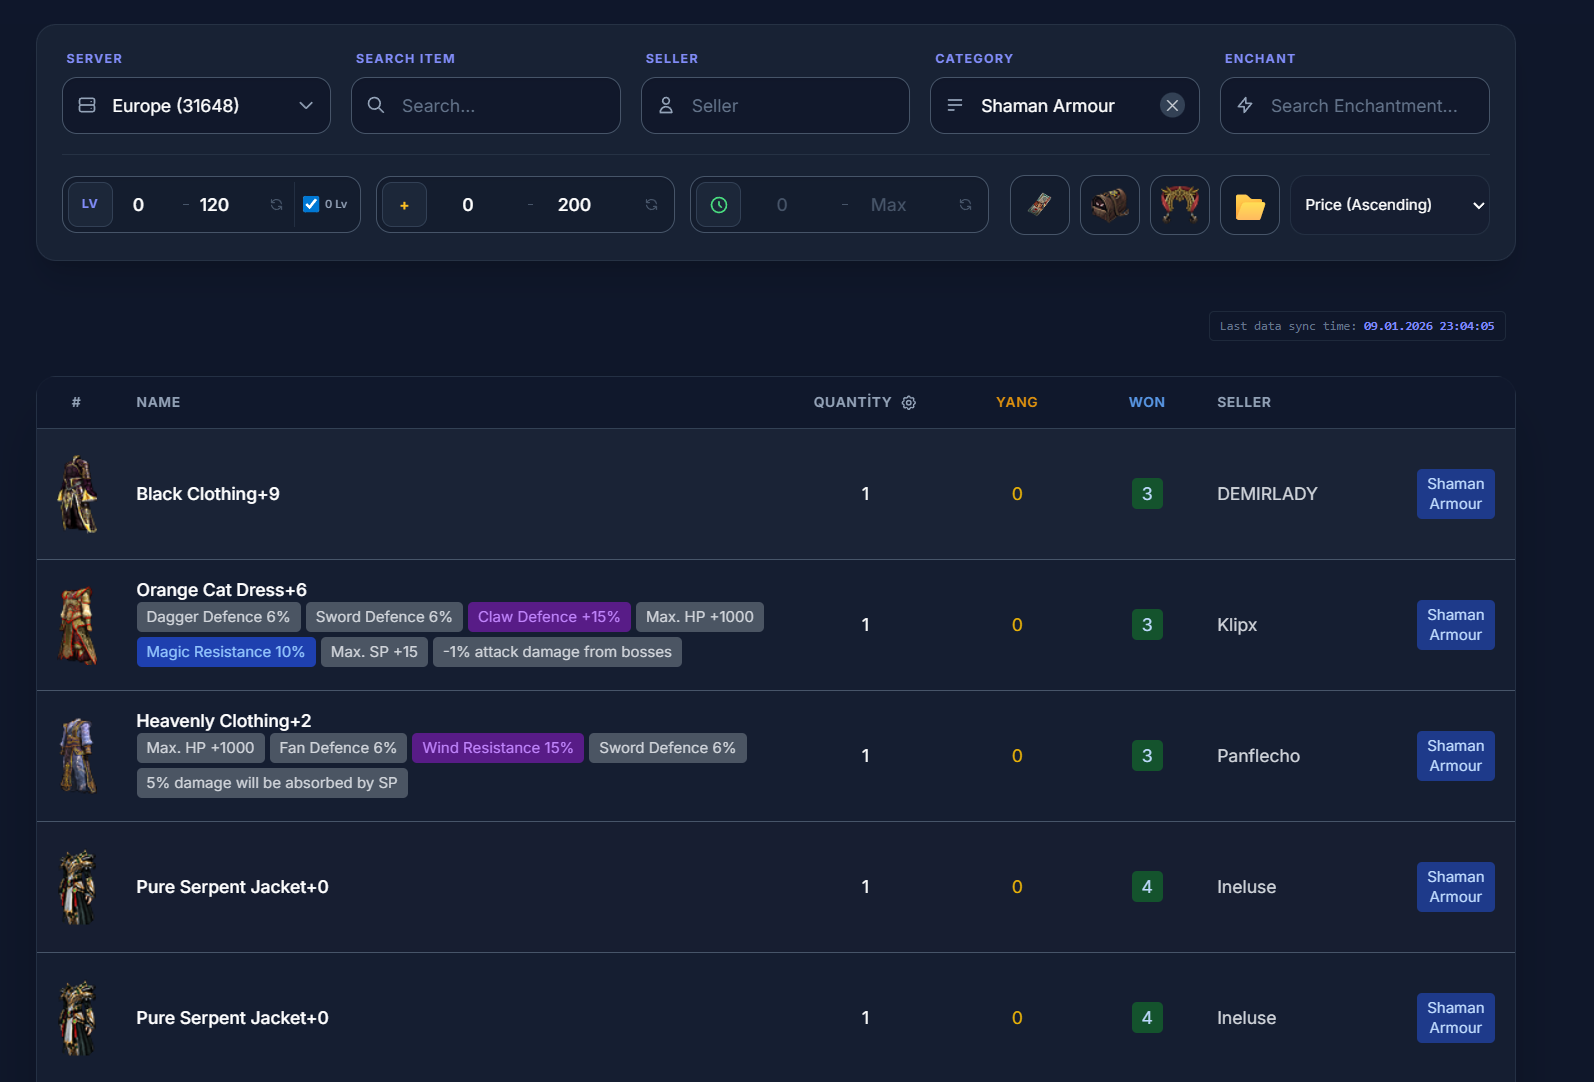
\includegraphics[width=0.7\linewidth]{metin2alerts_market.png}
    \caption{Screenshot of the Metin2Alerts marketplace showing listed items, prices, and item attributes}
    \label{fig:metin2alerts_market}
\end{figure}


\subsection{Currency model (Yang and Won)}
Prices are expressed using two in-game currencies:
\begin{itemize}
  \item \textbf{Yang}: the most common currency used for everyday trades (``small change'').
  \item \textbf{Won}: higher denomination currency used for expensive items (``big bills'').
\end{itemize}
In the warehouse, both are stored so analyses can handle cheap and expensive items consistently.

\subsection{Objects of analysis and granularity}
The primary object of analysis is a \textbf{market listing snapshot}. A snapshot represents the market state at a given capture time.
For decision support, we analyze the market at multiple granularities:
\begin{itemize}
  \item \textbf{Listing level}: seller, server, prices (Yang/Won), and quantity.
  \item \textbf{Item identity level}: 
  the \texttt{vnum} item identifier for grouping and trend tracking.
  \item \textbf{Item instance properties}: enhancement level, sockets, and bonus attributes that influence the price.
  \item \textbf{Time level}: daily time dimension for trends and volatility metrics.
\end{itemize}

\subsection{Key measures and KPIs}
The system targets measurable indicators needed for market decisions:
\begin{itemize}
  \item \textbf{Price statistics}: average/min/max prices per item and period.
  \item \textbf{Trend and volatility}: trend direction (up/down/stable) and volatility score.
  \item \textbf{Deal detection}: undervaluation percentage, potential profit, and confidence score.
  \item \textbf{Attribute-driven value}: rarity score and value multipliers from bonuses.
\end{itemize}

\section{Decision-making issues}
Players and traders face several recurring decision problems:
\begin{itemize}
  \item \textbf{Fair pricing}: determining whether a listed item price is normal, expensive, or a bargain.
  \item \textbf{Trend detection}: understanding if an item is going up/down over time.
  \item \textbf{Attribute impact}: quantifying how bonuses/enchantments and enhancement level affect price.
  \item \textbf{Server differences}: comparing the same item across different servers.
\end{itemize}

\section{Stakeholders}
\begin{itemize}
  \item \textbf{Casual players}: want quick guidance to avoid overpaying.
  \item \textbf{Traders}: search for undervalued listings and arbitrage opportunities.
  \item \textbf{Guild leaders}: plan equipment upgrades and budget planning for members.
  \item \textbf{Market analysts}: study the economy dynamics and item liquidity.
\end{itemize}

\begin{questionbox}
\begin{enumerate}
  \item What are the \textbf{top most expensive items} on a given server in average Yang price?
  \item For a given item (\texttt{vnum}), what is the \textbf{price evolution over time}?
  \item Which listings look \textbf{undervalued} compared to an estimated fair value?
  \item How do \textbf{bonuses/enchantments} and \textbf{enhancement level} influence price?
  \item How do prices differ between \textbf{Server 502} and \textbf{Server 71}?
\end{enumerate}
\end{questionbox}


\chapter{Data sources}

\section{Identification of data sources}

\begin{challengebox}
	\textbf{How to access the data (options considered).} \\[0.25em]
To build a warehouse, we needed a reliable way to collect market listings at scale.
We considered three approaches:
\begin{enumerate}
	\item \textbf{In-game memory scanning} to read shop states directly from the game process.
	\textit{Rejected:} high risk of violating game rules and getting banned.

	\item \textbf{Classic HTML web scraping} of \url{https://metin2alerts.com/store/}.
	\textit{Rejected:} the site is paginated and the market is massive.
	At the time of writing, the market contains roughly \textbf{1697 pages} and \textbf{31122 items}.
	Scraping would be slow, brittle, and could still produce messy/incomplete data.

	\item \textbf{Client-side reverse engineering (chosen)}: observe the website network traffic to identify the real data endpoints.
	\\
		\textit{Accepted:} this approach retrieves structured JSON directly (consistent format, fast to download, and easier to validate).
\end{enumerate}

	\textbf{Outcome.} \\[0.25em]

By reverse engineering the client network requests, we discovered that the site fetches market listings from server-specific JSON snapshots and enriches them with several reference JSON files.
This discovery directly influenced the warehouse design and the ETL strategy (which fields to keep, which reference files to join, and which attributes to normalize).
\end{challengebox}

\section{Description of sources used}
The project uses three categories of sources:
\begin{itemize}
  \item \textbf{Web JSON (market snapshots)} from Metin2Alerts: server-specific listing snapshots.
  \item \textbf{Web JSON (static reference)} from Metin2Alerts: dictionaries and metadata needed to interpret the listings.
  \item \textbf{PostgreSQL warehouse}: the structured analytical store (facts, dimensions, aggregates).
\end{itemize}

\section{Type of data}
\begin{itemize}
  \item Semi-structured data: JSON (market listings and reference files).
  \item Structured data: PostgreSQL tables (facts, dimensions, aggregates, views).
\end{itemize}

Once we decided that client-side reverse engineering was the safest and most scalable acquisition method, the next question was:
	\textit{ what exactly does the website download, and how are the files connected?}

By observing the network traffic of \url{https://metin2alerts.com/store/}, we found that the website relies on:
\begin{itemize}
  \item \textbf{Market snapshots}: large JSON arrays containing the actual listings for a given server.
  \item \textbf{Reference files}: smaller JSON files that provide meaning and labels (names, bonus/stat meanings, UI strings, etc.).
\end{itemize}

\begin{figure}[H]
    \centering
    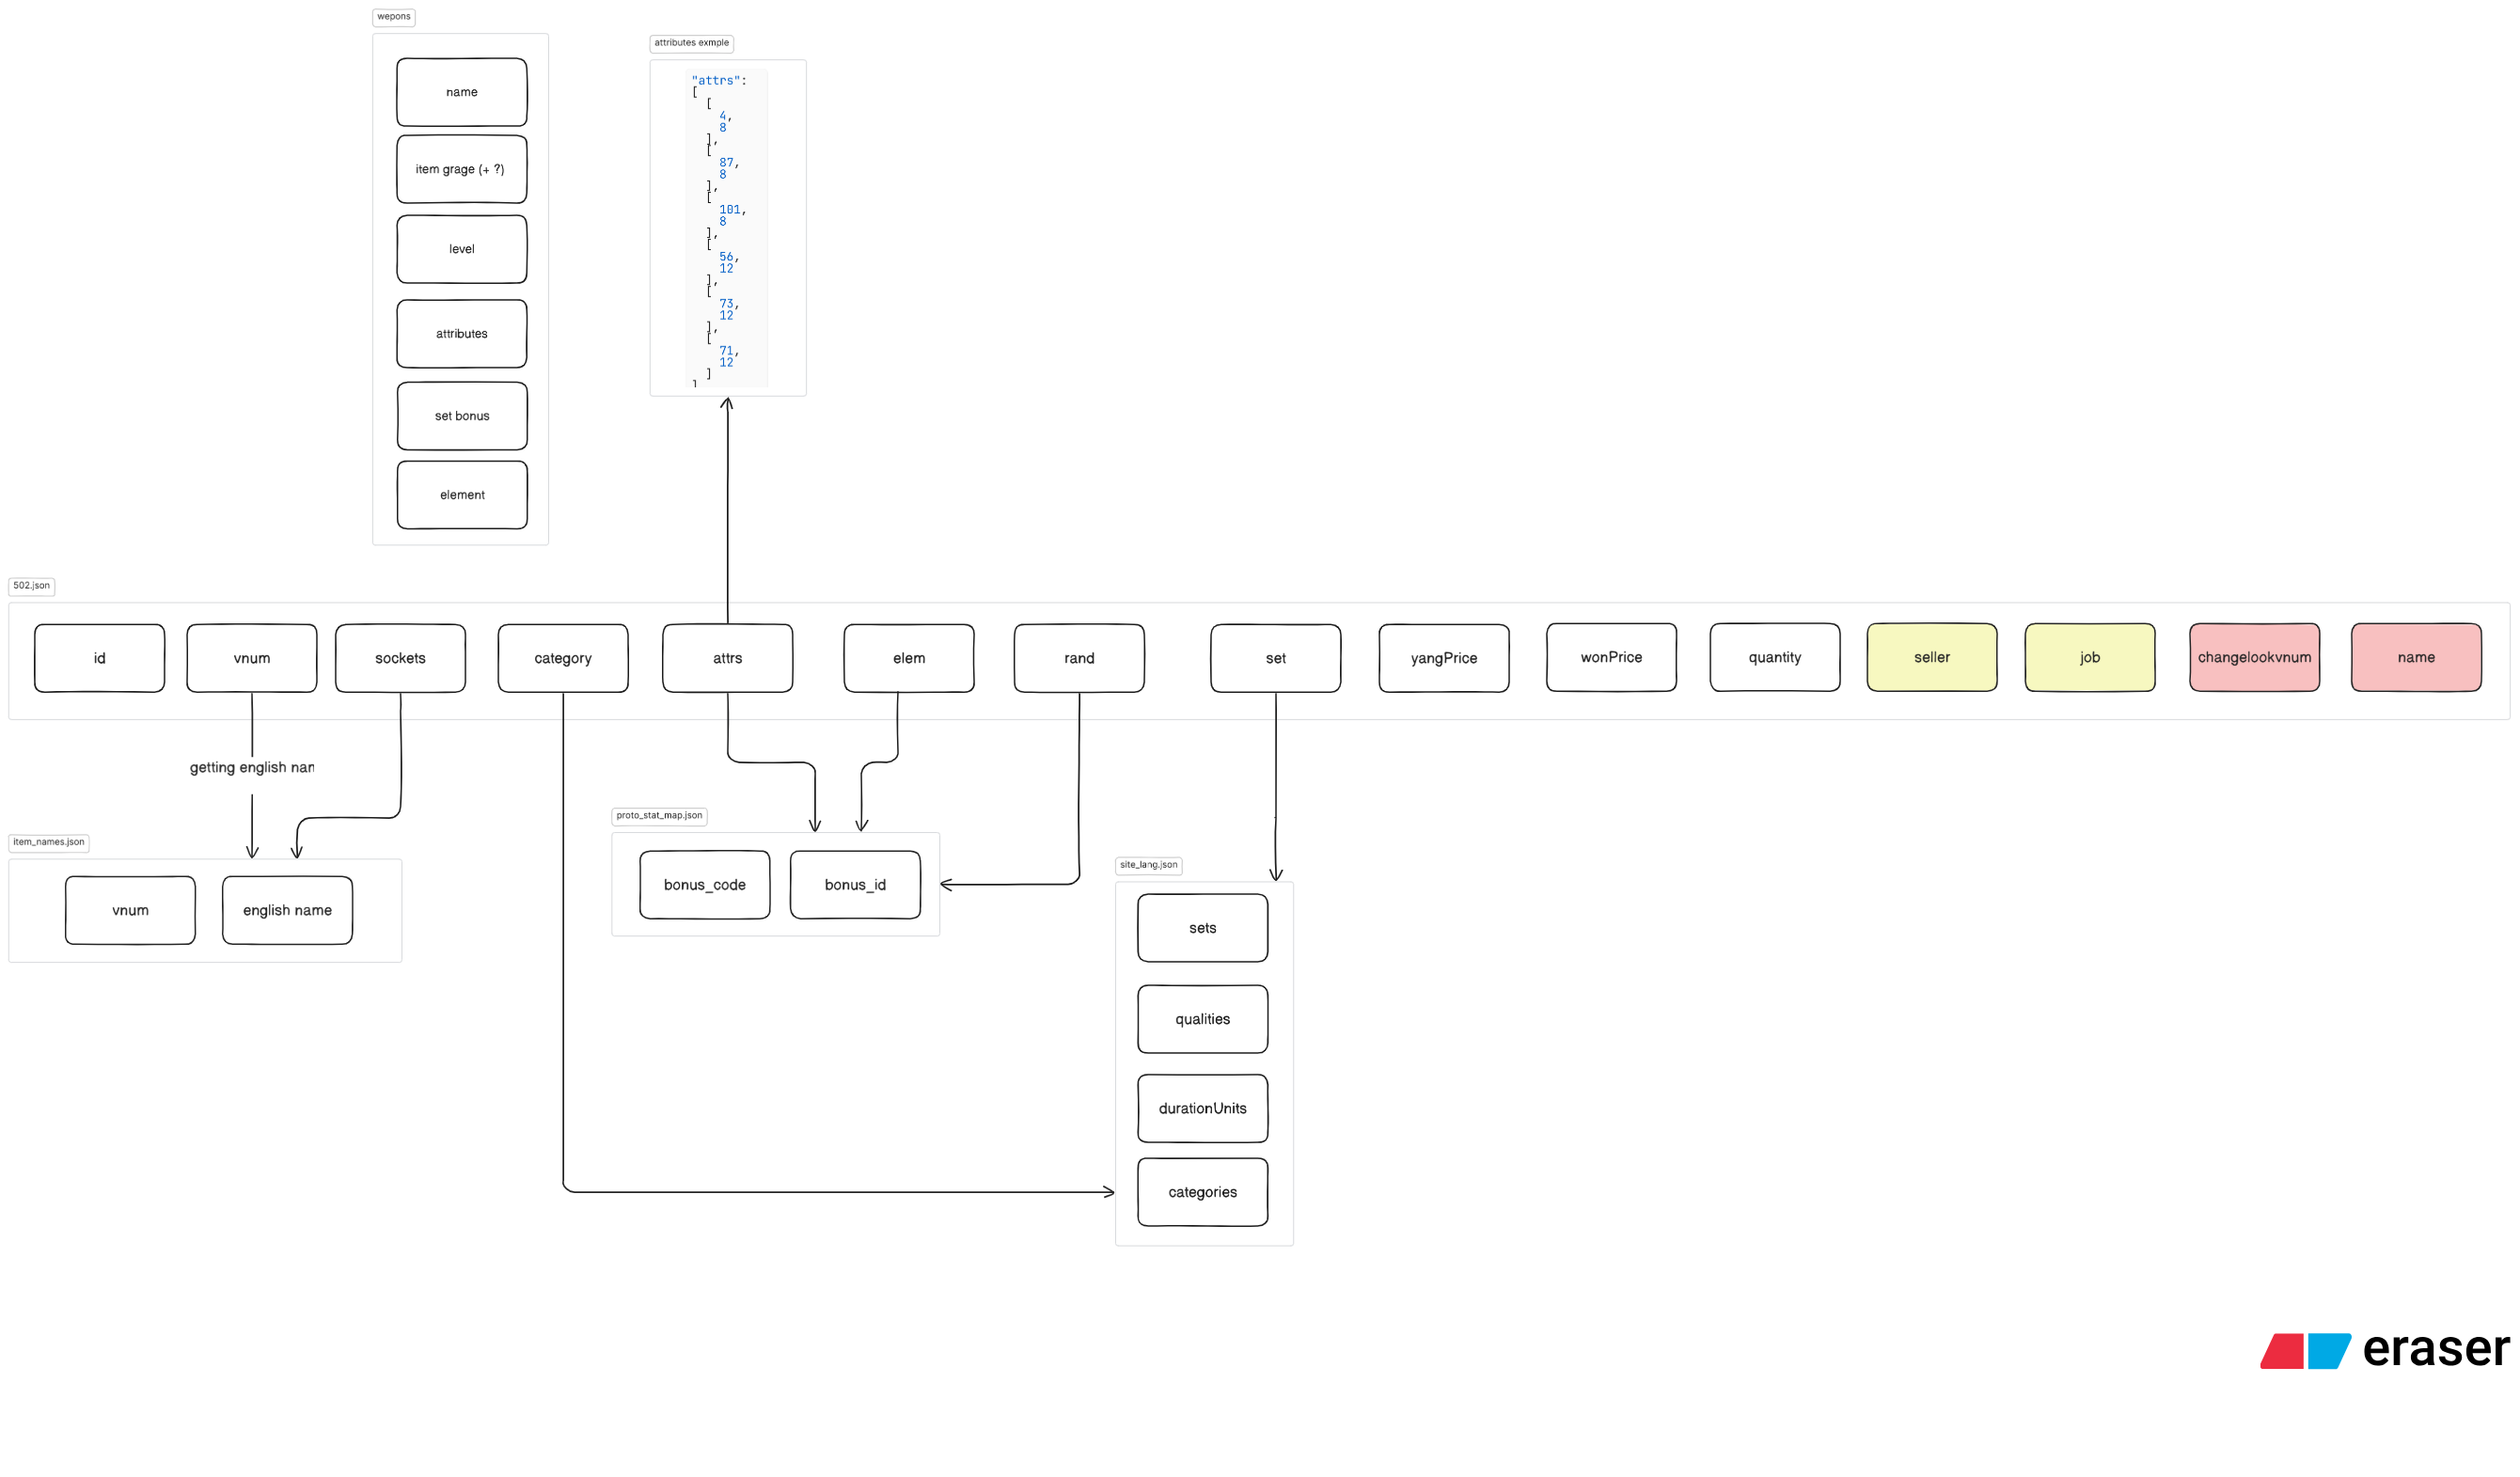
\includegraphics[width=0.92\linewidth]{filesRs.png}
    \caption{Relationships Between Market JSON and Reference JSON Files}
    \label{fig:json-relationships}
\end{figure}


\section{Discovered JSON files and their roles}
\subsection{Market data (large, server-specific)}
The website fetches market listings as a JSON snapshot per server:
\begin{itemize}
  \item \texttt{https://metin2alerts.com/store/public/data/502.json} (Europe)
  \item \texttt{https://metin2alerts.com/store/public/data/71.json} (Teutonia)
\end{itemize}
Each file contains a large array of listings, where each listing includes identity fields (like \texttt{vnum}), seller information, prices, and detailed item attributes.

\subsection{Static reference files (small, meaning/labels)}
The website also relies on several reference JSON files (English in our project) to interpret the listing payload.
We synchronize these files once and reuse them throughout the ETL:

\begin{table}[!ht]
\centering
\caption{Reference JSON files used to interpret listings}
\begin{tabularx}{\linewidth}{@{}lX@{}}
	\toprule
	\textbf{File} & \textbf{Purpose (observed)} \\
\midrule
	\texttt{/m2\_data/en/stat\_map.json} & Human-readable mapping for a subset of game stats/labels.
\\
	\texttt{/m2\_data/proto\_stat\_map.json} & Maps stat/bonus identifiers to their meaning (used to interpret \texttt{attrs}, \texttt{rand}, and \texttt{elem}).
\\
	\texttt{/m2\_data/item\_proto.json} & Base item metadata (type/subtype and proto fields that help decode weapon/armor stats).
\\
	\texttt{/m2\_data/en/item\_names.json} & Stable English item names indexed by \texttt{vnum} (used to avoid localization issues).
\\
	\texttt{/m2\_data/item\_icon.json} & Maps items to icon filenames for UI/display.
\\
	\texttt{/m2\_data/en/itemdesc.json} & Item descriptions (textual reference).
\\
	\texttt{/m2\_data/en/site\_lang.json} & UI strings and enumerations (including labels for special ``set'' titles).
\\
	\texttt{/m2\_data/en/mob\_names.json} & Monster names (auxiliary reference).
\\
	\texttt{/m2\_data/en/pet\_skills.json} & Pet skills reference (auxiliary reference).
\\
\bottomrule
\end{tabularx}
\end{table}

\section{Reverse engineered listing fields (market payload)}
After collecting the snapshot JSON, we still needed to interpret the meaning of the fields.
The following mapping summarizes the key fields used by the ETL.

\begin{longtable}{@{}p{0.22\linewidth}p{0.73\linewidth}@{}}
\caption{Market listing fields and interpreted semantics}\label{tab:market-payload-fields}\\
		\toprule
		\textbf{Field} & \textbf{Meaning and usage in the warehouse} \\
\midrule
\endfirsthead
		\toprule
		\textbf{Field} & \textbf{Meaning and usage in the warehouse} \\
\midrule
\endhead
\bottomrule
\endfoot

	\texttt{vnum} & \textbf{Virtual number}: the item identifier. All items with the same base identity share the same \texttt{vnum}. Used as the natural key for \texttt{dim\_item}. \\

	\texttt{name} & The displayed name in the market payload (often localized, e.g., German). \textbf{Ignored for analysis labels}; we use English mapping from \texttt{item\_names.json}. \\

	\texttt{seller} & Seller name (listing context). Stored in fact tables for analysis (seller behavior, clustering, etc.). \\

	\texttt{yangPrice} & Price in \textbf{Yang} (small denomination). Stored as \texttt{transaction\_price\_yang}. \\

	\texttt{wonPrice} & Price in \textbf{Won} (large denomination). Stored as \texttt{transaction\_price\_won}. \\

	\texttt{quantity} & Quantity listed. Meaningful mainly for stackable items; for non-stackable items it is typically 1. \\

	\texttt{job} & A class/job identifier associated with the listing context. Stored as \texttt{job\_id} for server-level and class-level filtering. \\

	\texttt{attrs} & Attributes (bonuses) array. Each element is a pair \texttt{[bonus\_id, bonus\_value]}. These are normalized into up to 7 attribute slots in \texttt{fact\_item\_attributes}. \\

	\texttt{sockets} & Array of socketed stones (typically stone \texttt{vnum}s). Stored to allow filtering and valuation heuristics. \\

	\texttt{rand} & Random bonus list (same structure as \texttt{attrs}), commonly observed on higher-level items. Treated as attributes but marked internally as random when needed. \\

	\texttt{set} & Special set/title flag (one of a finite set of possibilities). Labels are derived from \texttt{site\_lang.json}. \\

	\texttt{elem} & Element info. Observed structure: \texttt{[elem\_bonus\_id, primary\_values, secondary\_values]}. In practice we keep the primary list and compute the total power as the sum of its values; the secondary list is ignored for our KPIs. The element bonus id meaning is taken from \texttt{proto\_stat\_map.json}. \\

	\texttt{changelookvnum} & Appearance override: if non-zero, the item is visually changed to another \texttt{vnum}. Useful for UI and some filtering logic. \\

\end{longtable}

\section{Why the correlations matter}
The warehouse design and ETL steps depend directly on these correlations:
\begin{itemize}
  \item \textbf{Stable naming}: \texttt{vnum} from the market snapshot must be joined with \texttt{item\_names.json} to obtain a consistent English label.
  \item \textbf{Bonus semantics}: \texttt{attrs/rand/elem} only become meaningful after mapping IDs using \texttt{proto\_stat\_map.json}.
  \item \textbf{Type-aware parsing}: base item type/subtype and proto values from \texttt{item\_proto.json} influence how we interpret weapon/armor stats and which facts/dimensions are populated.
\end{itemize}
Because of this dependency chain, we treat reference files as first-class sources and synchronize them before processing market snapshots.

\begin{riskbox}
\textbf{Data quality issues encountered and mitigations:}
\begin{itemize}
  \item \textbf{Localization / inconsistent item names}: market payload may include localized names. 
  Mitigation: enforce English naming via synced reference mapping (vnum $\rightarrow$ name).

  \item \textbf{Schema uncertainty}: attribute arrays, sockets, and nested fields vary by item type. 
  Mitigation: reverse engineer and normalize into stable columns (e.g., 7 attribute slots) and computed metrics.

  \item \textbf{Duplicates}: exact replicas may appear multiple times in one snapshot. 
  Mitigation: deduplicate identical listings before loading.

  \item \textbf{Temporal bias}: snapshots represent the market at fetch time. Some listings may persist across time. 
  Mitigation: use a time dimension and batch timestamps to track snapshots consistently.
\end{itemize}
\end{riskbox}

\placeholderfigure{Example Market JSON Structure (annotated)}{0.92\linewidth}{5.5cm}


\chapter{Data Warehouse Design}

\section{Choice of schema type}
Based on the available sources (market snapshots + reference JSON files described in the previous chapter), we selected a \textbf{constellation schema} (multiple fact tables sharing common dimensions). 
This design supports different analytical perspectives (transactions, attributes, undervalued detection) while reusing core dimensions such as \texttt{dim\_item} and \texttt{dim\_time}.

\section{Multidimensional model diagram}
\begin{figure}[H]
    \centering
    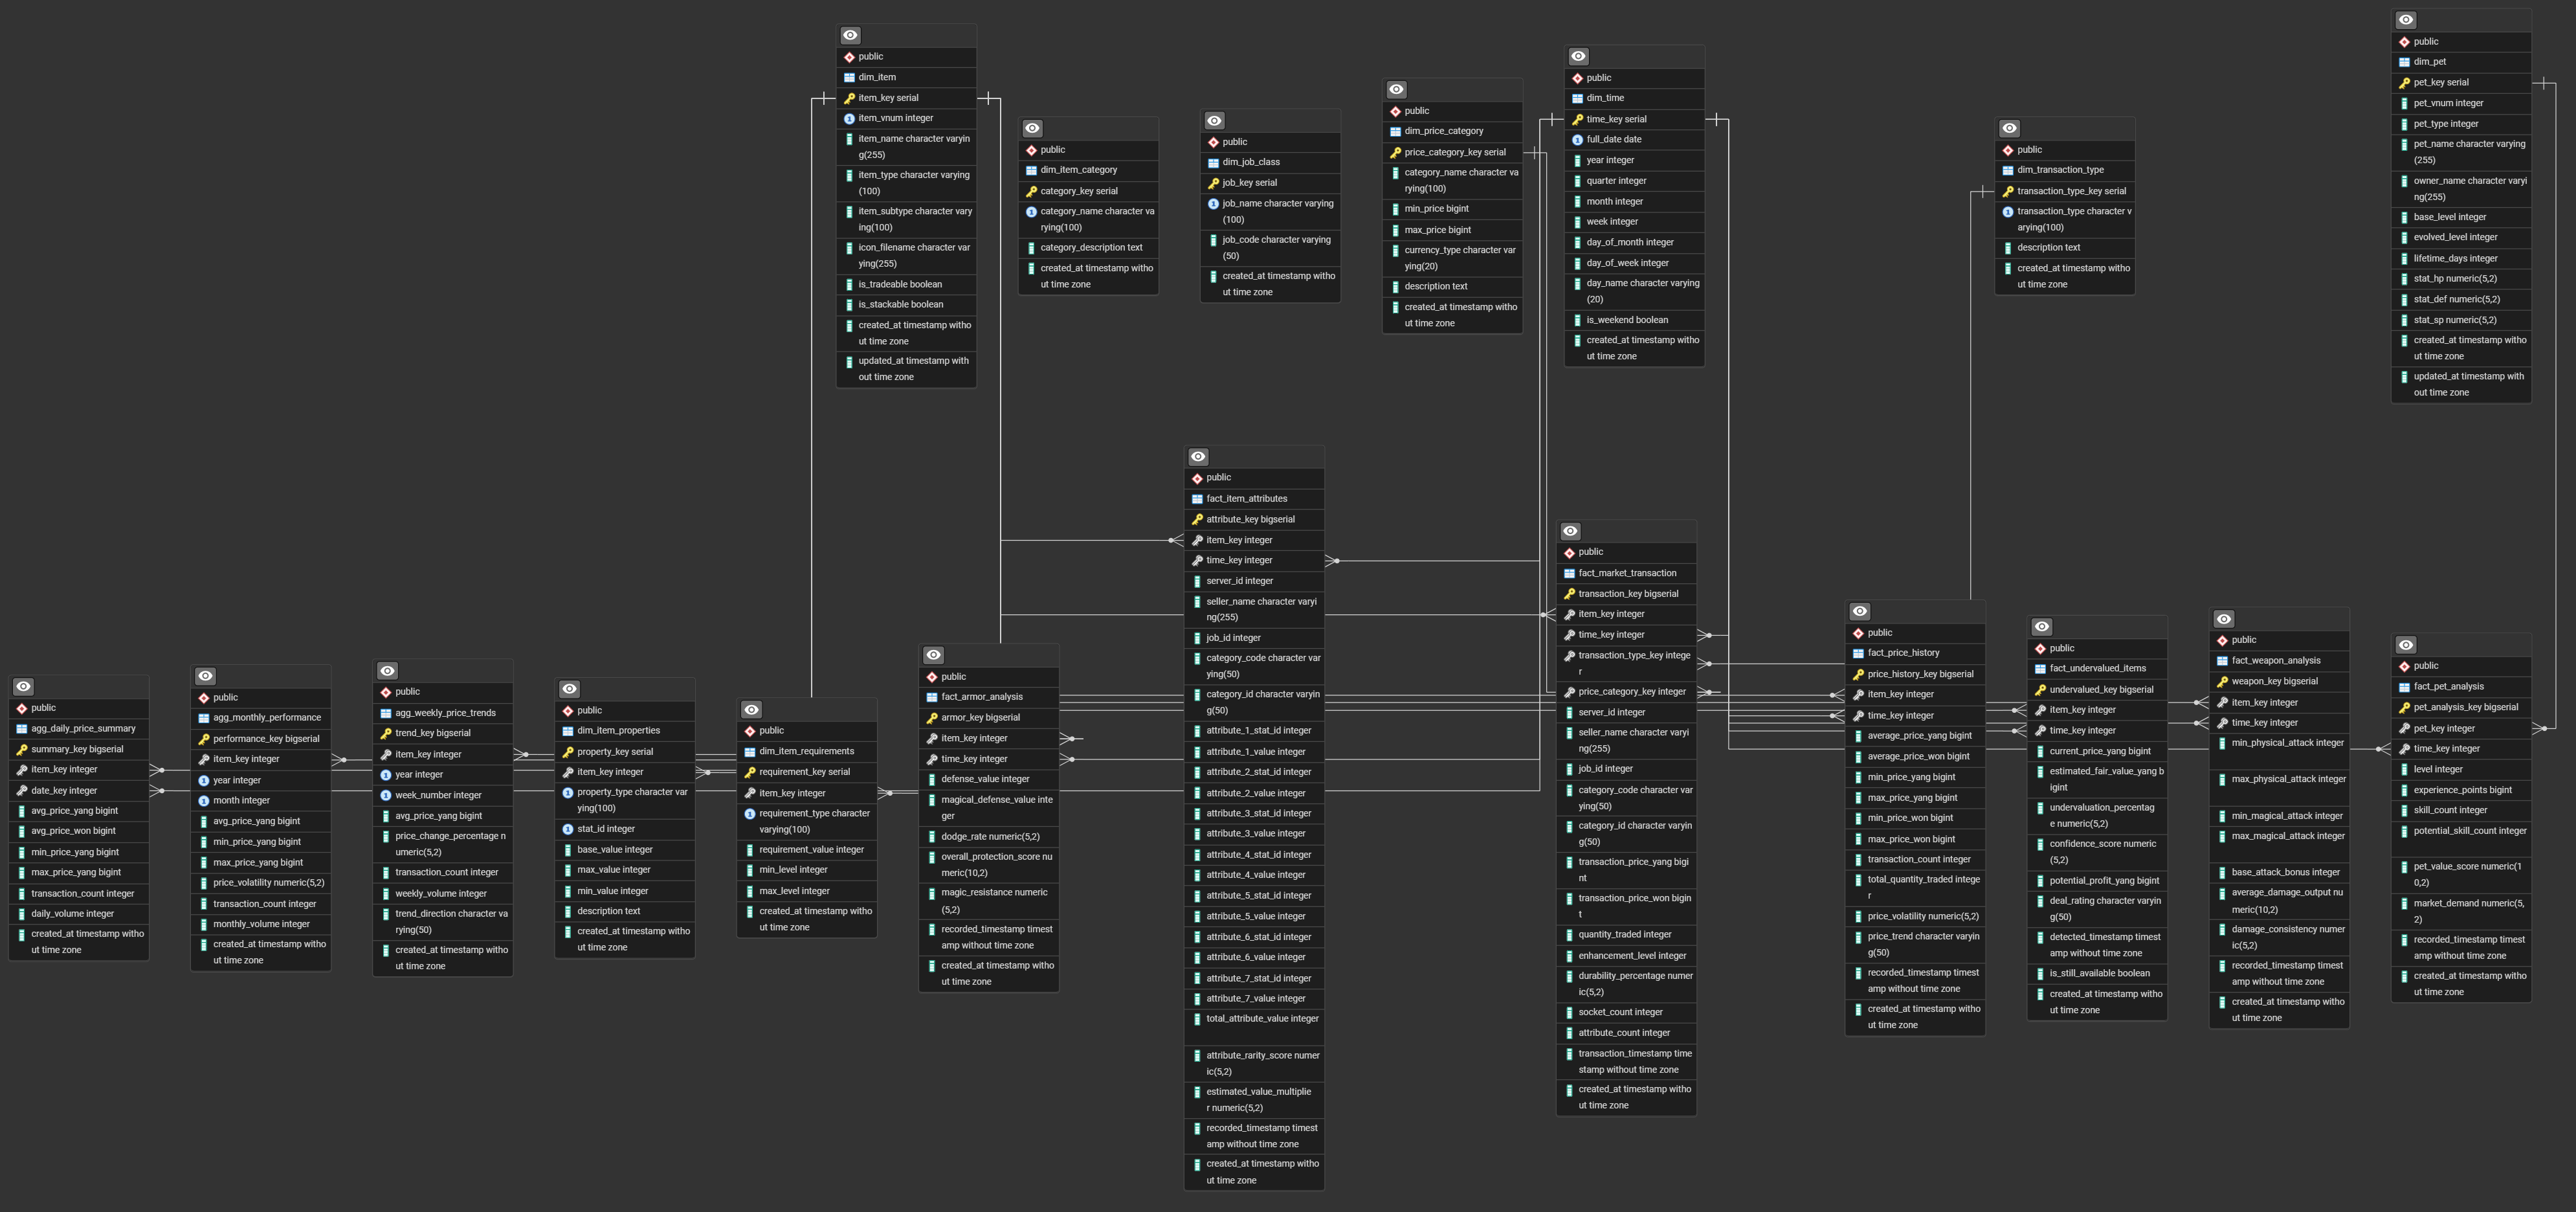
\includegraphics[width=0.92\linewidth]{Schema.png}
    \caption{Constellation schema overview (core tables used for analysis).}
    \label{fig:json-relationships}
\end{figure}


\section{Description of fact tables and dimensions}
\subsection{Core dimensions}
\begin{table}[!ht]
\centering
\caption{Main dimensions (excerpt)}
\begin{tabularx}{\linewidth}{@{}lX@{}}
\toprule
\textbf{Dimension} & \textbf{Role in analysis} \\
\midrule
\texttt{dim\_item} & Item reference: vnum, English name, type/subtype, tradeable/stackable flags. \\
\texttt{dim\_time} & Time axis for trends, daily/weekly/monthly aggregations. \\
\texttt{dim\_transaction\_type} & Separates listing/transaction semantics (when applicable). \\
\texttt{dim\_price\_category} & Enables bucketed analysis by price range. \\
\bottomrule
\end{tabularx}
\end{table}

\subsection{Main facts}
\begin{table}[!ht]
\centering
\caption{Main fact tables (excerpt)}
\begin{tabularx}{\linewidth}{@{}lX@{}}
\toprule
\textbf{Fact} & \textbf{Measures / KPIs} \\
\midrule
\texttt{fact\_market\_transaction} & transaction\_price\_yang/won, quantity, enhancement\_level; listing context (server, seller, category). \\
\texttt{fact\_item\_attributes} & up to 7 attribute stat/value pairs; rarity score; estimated value multiplier. \\
\texttt{fact\_price\_history} & average/min/max prices per day; volatility; trend direction. \\
\texttt{fact\_undervalued\_items} & undervaluation\%, confidence score, potential profit, deal rating. \\
\bottomrule
\end{tabularx}
\end{table}

\placeholderfigure{Full Multidimensional Model Diagram (detailed)}{0.92\linewidth}{6cm}


\chapter{ETL Process}

\section{Overall process architecture}
The ETL is fully automated and is triggered by the backend sync loop:
the service periodically fetches market JSON for the allowed servers (Europe and Teutonia), detects changes via a hash, and executes the ETL only when a new snapshot is detected.

\begin{itemize}
  \item \textbf{Scheduler / change detection:} \texttt{sync/auto\_sync.py}
  \item \textbf{ETL orchestrator:} \texttt{etl/pipeline.py}
  \item \textbf{Extract:} \texttt{etl/extractor.py} + \texttt{etl/cleaning.py}
  \item \textbf{Transform:} \texttt{etl/transformer.py}
  \item \textbf{Load (pygramETL + PostgreSQL):} \texttt{etl/loader.py}
\end{itemize}

\placeholderfigure{ETL Flow (Extract \textrightarrow Transform \textrightarrow Load)}{0.92\linewidth}{5.5cm}

\section{Detailed description of ETL steps}
\subsection{Extract}
	extbf{Goal:} Convert semi-structured market JSON into consistent Python domain objects.
\begin{itemize}
  \item Fetch market payload (JSON array) from the external source.
  \item De-duplicate exact duplicate listings in one fetch (prevents inflated counts).
  \item Clean payload shape and types (e.g., missing arrays, wrong types) using \texttt{etl/cleaning.py}.
  \item Parse each listing into a \texttt{MarketItem} (\texttt{models/market\_models.py}) using \texttt{etl/extractor.py}:
  vnum, item type/subtype, sockets, attributes (regular + random), durability, enhancement, price (won + yang).
  \item Enrich listing context fields used for filtering and analysis:
  	exttt{server\_id}, \texttt{seller\_name}, \texttt{job\_id}, \texttt{category\_code}, \texttt{category\_id}, \texttt{quantity}.
  \item \textbf{English naming:} the extractor prefers English item names from synced static reference files
  (\texttt{data/external/m2\_data/en/item\_names.json}) to ensure stable labels across servers/locales.
\end{itemize}

\subsection{Transform}
	extbf{Goal:} Apply business rules and produce dimension/fact records ready for a constellation schema.
\begin{itemize}
  \item Create a single \textbf{batch timestamp} for the full snapshot (\texttt{etl/pipeline.py}).
  This makes it possible to join facts for the same snapshot and avoids mixing partial loads.
  \item Normalize descriptive fields (e.g., strip HTML tags from names) using \texttt{DataTransformer.normalize\_item\_name}.
  \item Build dimension rows (\texttt{etl/transformer.py}):
  	exttt{dim\_item} (stable item identity) and \texttt{dim\_time} (calendar attributes).
  \item Build property rows (\texttt{dim\_item\_properties}) from parsed stats/bonuses so equipment analysis can group by bonuses.
  \item Build fact rows for each listing:
  \begin{itemize}
    \item \texttt{fact\_market\_transaction}: prices, quantity, enhancement, durability, sockets, attribute count + listing context.
    \item \texttt{fact\_item\_attributes}: up to 7 attribute slots (stat/value), rarity score and derived multipliers.
  \end{itemize}
  \item Compute decision-support KPIs:
  \begin{itemize}
    \item \textbf{Estimated fair value:} \texttt{DataTransformer.estimate\_item\_fair\_value} (intrinsic model).
    \item \textbf{Undervaluation detection:} \texttt{DataTransformer.detect\_undervalued\_item} produces \texttt{fact\_undervalued\_items}
    with percentage, profit, confidence score, and a deal rating.
  \end{itemize}
\end{itemize}

\subsection{Load (pygramETL)}
	extbf{Goal:} Load records into PostgreSQL using \textbf{pygramETL} abstractions (dimensions + facts).
\begin{itemize}
  \item \textbf{When and where we connect with pygramETL:}
  the connection is created during the load phase inside \texttt{WarehouseLoader.connect()} (\texttt{etl/loader.py}).
  \item \textbf{How it connects:}
  \begin{itemize}
    \item Connect to PostgreSQL using \texttt{psycopg2.connect(connection\_string)}.
    \item Wrap the DB connection using \texttt{pygrametl.ConnectionWrapper} and set it as default via \texttt{dwconn.setasdefault()}.
    \item Initialize pygramETL table objects in \texttt{WarehouseLoader.\_setup\_pygrametl\_tables()}:
    	exttt{CachedDimension} for \texttt{dim\_item}, \texttt{dim\_time}, \texttt{dim\_transaction\_type} and \texttt{FactTable} for facts.
  \end{itemize}
  \item Use \texttt{CachedDimension.ensure()} to insert-or-get dimension rows and obtain surrogate keys.
  \item Insert facts with foreign keys using \texttt{FactTable.insert()}.
  \item Commit per stage and rollback on error (keeps warehouse consistent).
\end{itemize}

\begin{challengebox}
	extbf{Why pygramETL?} \newline
pygramETL provides a clean loading layer for dimensional models:
\begin{itemize}
  \item \textbf{Idempotent dimensions:} \texttt{ensure()} avoids duplicate dimension rows when the same item appears across many snapshots.
  \item \textbf{Surrogate key handling:} dimensions return surrogate keys directly, simplifying fact inserts.
  \item \textbf{Caching:} \texttt{CachedDimension} speeds up repeated lookups for popular items.
\end{itemize}
\end{challengebox}

\section{Justification of transformations applied}
\begin{itemize}
  \item \textbf{English normalization}: stable labels across servers/locales; better grouping in dashboards.
  \item \textbf{Dimensional modeling}: separates stable descriptions (dimensions) from changing measures (facts).
  \item \textbf{Batch timestamps}: consistent snapshot alignment across facts (transactions + attributes + undervaluation).
  \item \textbf{Derived KPIs}: turns raw prices into decision-ready metrics (estimated value, confidence, profit).
\end{itemize}

\begin{challengebox}
\textbf{Reverse engineering (API + JSON).} \\[0.25em]
After discovering the JSON endpoints by observing client network calls, we still had to interpret the payload:
\begin{itemize}
  \item Identify which fields represent item identity vs. listing identity.
  \item Decode attribute arrays and their stat/value meaning.
  \item Handle missing or item-type-specific fields safely.
\end{itemize}
This reverse engineering step was essential to create a stable schema suitable for a warehouse.
\end{challengebox}


\chapter{Implementation}

\section{Python code (ETL + visualization)}
The system is implemented in Python with a clear separation of concerns:
\begin{itemize}
  \item \textbf{Sync}: periodic fetch + state tracking + change detection.
  \item \textbf{ETL}: extraction, transformation, loading into PostgreSQL.
  \item \textbf{Reporting}: Matplotlib dashboards computed from warehouse queries.
\end{itemize}

\section{Application features (API + React web application)}
This project includes a complete decision-support application on top of the warehouse:
\begin{itemize}
  \item A \textbf{FastAPI backend} that exposes analytical endpoints and runs the automatic sync + ETL loop at startup.
  \item A \textbf{web dashboard} (Vite + React) that lets users search items, plot price history, analyze equipment bonuses, and browse undervalued deals.
\end{itemize}

UI screenshots are consolidated in Chapter~7.

\subsection{Automation and scheduling}
A periodic loop runs inside the backend service. It fetches market data for the allowed servers, compares a hash of the normalized payload, and triggers ETL only when the payload changes.

\placeholderfigure{Automation Loop Timeline (every 10 minutes)}{0.92\linewidth}{5cm}

\subsection{Loading with pygramETL (concept)}
The loader uses pygramETL to manage dimensions and facts through reusable abstractions.

\begin{lstlisting}[style=python,caption={Simplified loading pattern with pygramETL (dimension ensure + fact insert)}]
# 1) Ensure dimension exists and get surrogate key
item_key = dim_item.ensure({
    "item_vnum": vnum,
    "item_name": item_name,
    "item_type": item_type,
})

# 2) Insert fact row referencing the dimension key
fact_market_transaction.insert({
    "item_key": item_key,
    "time_key": time_key,
    "transaction_type_key": trx_type_key,
    "transaction_price_yang": price_yang,
    "enhancement_level": plus,
    "transaction_timestamp": batch_timestamp,
})

dwconn.commit()
\end{lstlisting}

\subsection{Matplotlib dashboards}
Dashboards are generated by querying the warehouse (via Pandas) and plotting KPIs in Matplotlib.
\begin{itemize}
  \item Top items by average price.
  \item Distribution of undervalued deals by rating.
  \item Time-series plot of an item price history.
\end{itemize}

\placeholderfigure{Matplotlib KPI Dashboard Screenshot}{0.92\linewidth}{6cm}

\section{SQL scripts used}
\begin{itemize}
  \item Warehouse creation script: constellation schema (dimensions, facts, aggregates, indexes, views).
  \item Analytical queries used by dashboards (top items, deal ratings, price history).
\end{itemize}

\begin{table}[!ht]
\centering
\caption{Examples of SQL queries used for dashboards}
\begin{tabularx}{\linewidth}{@{}lX@{}}
\toprule
\textbf{KPI} & \textbf{Query idea (simplified)} \\
\midrule
Top expensive items & Average of \texttt{fact\_price\_history.average\_price\_yang} grouped by \texttt{dim\_item.item\_name}. \\
Deals by rating & Count of rows per \texttt{fact\_undervalued\_items.deal\_rating}. \\
Price history & Join \texttt{fact\_price\_history} with \texttt{dim\_time} and filter by item \texttt{vnum}. \\
\bottomrule
\end{tabularx}
\end{table}


\chapter{Dashboard and web application}

\section{Objective}
The warehouse is complemented by two user-facing layers:
\begin{itemize}
  \item a \textbf{server-rendered dashboard} implemented in Python (FastAPI + Jinja2 + Plotly) at \texttt{/dashboard},
  \item a \textbf{single-page web application} implemented with Vite + React, which consumes the backend APIs.
\end{itemize}
The goal is to translate warehouse facts (prices, attributes, deal detection) into a decision-support experience: quick price lookup, trend visualization, equipment bonus impact analysis, undervalued deals browsing, and rule-based alerts.

\section{Server-rendered dashboard (FastAPI + Plotly)}
The route \texttt{/dashboard} renders a single HTML page (template \texttt{api/templates/dashboard.html}) with interactive Plotly graphs.
It is useful for quick exploration without running the React app.

\subsection{Main features}
\begin{itemize}
  \item \textbf{Item search}: search by item name and select item \texttt{vnum} values.
  \item \textbf{Non-equipment price history}: plot min/avg price over time for one or more selected items.
  \item \textbf{Equipment analysis}: compute which bonuses correlate with higher prices ("premium") for a selected equipment \texttt{vnum}.
  \item \textbf{Equipment estimator}: estimate an equipment price from bonus pairs written as \texttt{stat:value} (example: \texttt{71:10,72:5}).
  \item \textbf{Deals list}: show undervalued opportunities from \texttt{fact\_undervalued\_items}.
\end{itemize}

\subsection{Screenshot}
\screenshotfigure{server_dashboard_plotly.png}{Server-rendered dashboard at \texttt{/dashboard}: Plotly visuals + search + deals.}

\section{React web application (Vite + React)}
The web UI is implemented as a React application (folder \texttt{web/}) with five pages: \textbf{Home}, \textbf{Alerts}, \textbf{Price history}, \textbf{Equipment}, and \textbf{Deals}.
It provides a more complete UX with navigation, filtering, and interactive Plotly charts.

\subsection{Navigation and theme}
The top navigation bar provides access to all pages and includes a light/dark theme toggle.
\screenshotfigure{web_nav.png}{Web UI: navigation bar and theme toggle.}

\subsection{Home: tracked items + price lookup}
The Home page is designed for continuous monitoring of a small list of items.
It starts with two defaults (\texttt{Voucher} \texttt{vnum=80017} and \texttt{Moonstone} \texttt{vnum=30618}) and lets the user add/remove tracked items.
The tracked list is saved locally in the browser (\texttt{localStorage}).

Each tracked item card shows:
\begin{itemize}
  \item latest minimum price (works even when there is only one day/sync group of data),
  \item average and maximum price, transaction count,
  \item a small server-generated chart (Matplotlib) returned as a base64 PNG.
\end{itemize}
\screenshotfigure{web_home.png}{Web UI: Home dashboard with tracked items and charts.}

\subsection{Price history: trends + filtering}
The Price history page allows selecting one or more items and plotting their time series (min and avg prices).
It supports decision-oriented filtering:
\begin{itemize}
  \item server selection (Europe 502 / Teutonia 71),
  \item category filtering,
  \item enchantment filtering with minimum values, combined with \textbf{AND} / \textbf{OR} matching.
\end{itemize}
The page also includes an \textbf{estimator for the current snapshot}, which proposes an estimated price given the active filters.
\screenshotfigure{web_price_history.png}{Web UI: Price history (multi-item Plotly chart + filters).}

\subsection{Equipment: bonus impact + estimator}
The Equipment page targets weapons/armor analysis.
It includes:
\begin{itemize}
  \item bonus impact ranking (top bonuses with the strongest observed price premium),
  \item an estimator that predicts price based on a typed bonus set (\texttt{stat:value} pairs).
\end{itemize}
\screenshotfigure{web_equipment.png}{Web UI: Equipment analysis (bonus impact + estimator).}

\subsection{Deals: undervalued opportunities}
The Deals page lists undervalued items computed by ETL (table \texttt{fact\_undervalued\_items}), including current price, estimated fair value, undervaluation percentage, potential profit, and deal rating.
\screenshotfigure{web_deals.png}{Web UI: Deals table from \texttt{fact\_undervalued\_items}.}

\subsection{Alerts: saved rules + monitoring}
The Alerts page provides a rule builder to query recent market listings.
Users can:
\begin{itemize}
  \item select servers,
  \item restrict items (optional \texttt{vnum} list),
  \item filter by max price, quantity, enhancement level range,
  \item filter by bonuses with \textbf{AND} / \textbf{OR} matching.
\end{itemize}
Alerts can be saved locally in the browser and reloaded later.
The page also provides a basic monitoring mode that periodically re-runs the query and displays new matches.
\screenshotfigure{web_alerts.png}{Web UI: Alerts builder with saved rules and monitoring.}

\section{KPI restitution (example outputs)}
The system also generates KPI plots from warehouse queries. Example figures produced by the Python dashboard scripts are included below.
\screenshotfigure{../outputs/kpi_top_items_avg_price.png}{KPI: Top items by average price (Matplotlib).}
\screenshotfigure{../outputs/kpi_deals_by_rating.png}{KPI: Undervalued deals by rating (Matplotlib).}
\screenshotfigure{../outputs/kpi_price_history_item_10001.png}{KPI: Price history example for one item (Matplotlib).}

\section{Screenshot checklist (files to add)}
To include real UI screenshots in the final PDF, export images and place them under \texttt{report/figures/} using the following filenames:
\begin{itemize}
  \item \texttt{web_nav.png}, \texttt{web_home.png}, \texttt{web_price_history.png}, \texttt{web_equipment.png}, \texttt{web_deals.png}, \texttt{web_alerts.png}
  \item \texttt{server_dashboard_plotly.png}
  \item \texttt{api_docs.png} (optional: Swagger UI at \texttt{/docs})
\end{itemize}
If a file is missing, the report will show a placeholder box instead of failing to compile.


\chapter{Conclusion}

\begin{conclusionbox}
\textbf{Project review.} \\[0.25em]
We built a complete decision-support pipeline: automated data collection, a PostgreSQL constellation warehouse, an ETL process (Extract/Transform/Load) in Python, and Matplotlib dashboards for KPI restitution.

\medskip
\textbf{Difficulties encountered.}
\begin{itemize}
  \item Accessing data at scale required client-side reverse engineering instead of brittle HTML scraping.
  \item JSON structure was non-trivial and required interpretation/normalization.
  \item Ensuring consistent English naming required reference data synchronization.
  \item Maintaining analytical consistency required batch timestamps and deduplication safeguards.
\end{itemize}

\medskip
\textbf{Prospects for improvement.}
\begin{itemize}
  \item Add richer slowly changing dimensions (SCD) for item metadata evolution.
  \item Improve incremental loading strategies and partitioning for very large history.
  \item Add additional data sources (e.g., CSV historical exports) to improve time coverage.
  \item Expand dashboards with more statistical models (seasonality, anomaly detection).
\end{itemize}
\end{conclusionbox}



\appendix
\chapter{Appendix}

\section{Repository map (for the examiner)}
\begin{itemize}
  \item ETL pipeline: \texttt{etl/pipeline.py}
  \item Extractor: \texttt{etl/extractor.py}
  \item Transformer: \texttt{etl/transformer.py}
  \item Loader (pygramETL): \texttt{etl/loader.py}
  \item SQL schema: \texttt{sql/constellation\_schema.sql}
  \item Matplotlib dashboards: \texttt{reporting/dashboard.py}
  \item Automation sync: \texttt{sync/auto\_sync.py}
\end{itemize}

\section{How to generate dashboard images (optional)}
Example commands:
\begin{lstlisting}[style=python,caption={Generate KPI images into an output folder}]
# From repository root:
# python -m reporting.dashboard --out repport/figures
# python -m reporting.dashboard --item-vnum 10001 --out repport/figures
\end{lstlisting}

\section{Notes on placeholders}
The report intentionally includes framed placeholders for diagrams and screenshots.
Replace them with real figures when available:
\begin{lstlisting}[style=python,caption={Replace placeholder with includegraphics}]
% \placeholderfigure{Title}{0.92\linewidth}{6cm}
% Replace with:
% \includegraphics[width=0.92\linewidth]{figures/my_image.png}
\end{lstlisting}



\end{document}
